\documentclass{beamer}

\usepackage[russian]{babel}
\usepackage[utf8]{inputenc}
\inputencoding{utf8}
\usepackage[normalem]{ulem}

\usepackage{subfigure}


% There are many different themes available for Beamer. A comprehensive
% list with examples is given here:
% http://deic.uab.es/~iblanes/beamer_gallery/index_by_theme.html
% You can uncomment the themes below if you would like to use a different
% one:
%\usetheme{AnnArbor}
%\usetheme{Antibes}
%\usetheme{Bergen}
%\usetheme{Berkeley}
%\usetheme{Berlin}
%\usetheme{Boadilla}
%\usetheme{boxes}
%\usetheme{CambridgeUS}
%\usetheme{Copenhagen}
%\usetheme{Darmstadt}
%\usetheme{default}
%\usetheme{Frankfurt}
%\usetheme{Goettingen}
%\usetheme{Hannover}
%\usetheme{Ilmenau}
%\usetheme{JuanLesPins}
%\usetheme{Luebeck}
\usetheme{Madrid}
%\usetheme{Malmoe}
%\usetheme{Marburg}
%\usetheme{Montpellier}
%\usetheme{PaloAlto}
%\usetheme{Pittsburgh}
%\usetheme{Rochester}
%\usetheme{Singapore}
%\usetheme{Szeged}
%\usetheme{Warsaw}

\title{Метод выпуклой оптимизации на квадрате}

\author{И.~Курузов\inst{1} \and Ф.~Стонякин\inst{1, 2}}
% - Give the names in the same order as the appear in the paper.
% - Use the \inst{?} command only if the authors have different
%   affiliation.

\institute[MIPT] % (optional, but mostly needed)
{
  \inst{1}%
Московский Физико-Технический Институт
  \and
  \inst{2}%
Крымский Федеральный Университет имени В.И.~Вернандского
}
% - Use the \inst command only if there are several affiliations.
% - Keep it simple, no one is interested in your street address.

\date{62-ая конференция МФТИ, 2019}
% - Either use conference name or its abbreviation.
% - Not really informative to the audience, more for people (including
%   yourself) who are reading the slides online

\subject{Theoretical Computer Science}
% This is only inserted into the PDF information catalog. Can be left
% out. 

% If you have a file called "university-logo-filename.xxx", where xxx
% is a graphic format that can be processed by latex or pdflatex,
% resp., then you can add a logo as follows:

% \pgfdeclareimage[height=0.5cm]{university-logo}{university-logo-filename}
% \logo{\pgfuseimage{university-logo}}

% Delete this, if you do not want the table of contents to pop up at
% the beginning of each subsection:
\AtBeginSubsection[]
{
  \begin{frame}<beamer>{Outline}
    \tableofcontents[currentsection,currentsubsection]
  \end{frame}
}

% Let's get started
\DeclareMathOperator{\sign}{sign}
\usepackage{tikz}
\begin{document}

\begin{frame}
  \titlepage
\end{frame}


\begin{frame}{Описание метода}
Задача:
$$\min_{(x,y)}\left\{f(x,y)|(x,y) \in Q\right\},$$
где $f$ выпулая функция, $Q = [a,b]\times[c, d]\in \mathbb{R}^2$.

\pause

\tikz{
    \draw (-1.5,1.5) -- (1.5,1.5) -- (1.5,-1.5) -- (-1.5,-1.5) -- (-1.5,1.5);
	\pause    
    \draw (-1.5,0) -- (1.5, 0);
    \pause
    \draw[red, ->] (-1, 0) -- (-1.1, 0.5);
    \node[below right] at (-1.1, 0.5){$\nabla f$}; 
    \pause
    \draw[dashed] (2.5,1.5) -- (5.5,1.5) -- (5.5,0) -- (2.5,0) -- (2.5,1.5);
    \draw (2.5,0) -- (5.5,0) -- (5.5,-1.5) -- (2.5,-1.5) -- (2.5,0);
	\pause    
    \draw (4, 0) -- (4, -1.5);
    \pause
    \draw[red, ->] (4, -0.75) -- (4.7, -0.8);
    \node[below right] at (4.1, -0.8){$\nabla f$};
    \pause
    \draw[dashed] (6.5, 0) -- (6.5, 1.5) -- (9.5, 1.5) -- (9.5, -1.5) -- (8, -1.5);
	\draw (6.5,0) -- (8, 0) -- (8, -1.5) -- (6.5, -1.5) -- (6.5, 0);
}
\end{frame}

\begin{frame}{План}
  \tableofcontents
  % You might wish to add the option [pausesections]
\end{frame}

% Section and subsections will appear in the presentation overview
% and table of contents.

\section{Стратегии для вспомогательных задач}

\begin{frame}{Стратегии}{Constant Estimate}
Пусть $f$ - $L$-липшецева с $M$-липшецевым градиентом.

Доказано, что следующей точности для одномерной задачи достаточно для достижения точности $\epsilon$ по функции исходной задачи:

$$\boxed{\delta \leq \frac{\epsilon}{2Ma(\sqrt{2}+\sqrt{5})(1-\frac{\epsilon}{La\sqrt{2}})}}$$
\pause
Сходимость по аргументу не гарантируется!
\end{frame}

\begin{frame}{Стратегии}{Current Gradient}
Хотим: выбрать прямоугольник, содержащий решение исходной задачи
\pause
Достаточно условия на знак:
    $$\sign f'_y(x_0) = \sign f'_y(x_{current})$$
\pause    
Усиленное условие
    $$|f'_y(x_0) - f'_y(x_{current})| \leq |f'_y(x_{current})|$$
\pause
В случае $M$-липшецевости градиента:
  $$\boxed{\delta \leq \frac{|f'_y(x_{current})|}{M}}$$
\end{frame}

\begin{frame}{Стратегии}{Малый градиент}
Что делать, если градиент мал?

\pause
\begin{block}{Small Gradient}
$f$ выпуклая функция с $M$-липшкецевым градиентом. Тогда точка $\textbf{x}$ - решение с точностью $\epsilon$, если

$$\|\nabla f(\textbf{x})\|\leq \frac{\epsilon}{a\sqrt{2}}, $$
где $a$ - размер квадрата.
\end{block}
\end{frame}

\section{Сходимость}

\begin{frame}{Сходимость}

Функция $f$ выпуклая функция. $Q$ - квадрат со стороной $a$.

\begin{block}{Сходимость}
Если функция $f$ $L$-липшецева, то для сходимости к решению с точностью $\epsilon$ по функции достаточно следующее количство итереций:
\begin{equation}\label{NI1}N = \left\lceil\log_2\frac{La\sqrt{2}}{\epsilon}\right\rceil.\end{equation}
\end{block}

\end{frame}

\begin{frame}{Сходимость}
\begin{block}{Сходимость}
Если

1. Функция $f$ имеет $M$-липшецев градиент

2. $\exists \textbf{x}^*\in Q: \nabla f(\textbf{x}^*) = \textbf{0}$

3. Стратегия обеспечивает сходимость по аргументу, 

то для сходимости к решению с точностью $\epsilon$ по функции достаточно следующее количство итереций:
\begin{equation}\label{NI3}N = \left\lceil\frac{1}{2}\log_2\frac{Ma^2}{4\epsilon}\right\rceil.\end{equation}
\end{block}

\end{frame}

\section{Двойственные задачи}
\begin{frame}{Двойственные задачи}{Задача}

Задача:

$$\min_{\textbf{x}\in \mathbb{R}^n} f(\textbf{x})$$
$$\text{s.t. } g_k(\textbf{x}) \leq 0, k = \overline{1,m}$$

где $f$ $\mu_f$-сильно выпуклая $L_f$-липшецева функция с $M_f$-липшецевым градиентом
, $g_k$  выпуклая $L_{g_k}$-липшецева функция с $M_{g_k}$-липшецевым градиентом для всех $k=\overline{1,m}$.
\end{frame}

\begin{frame}{Двойственные задачи}{Задача}
Двойственная задача с точностью до знака:

$$\min_{\lambda \in \mathbb{R}^m_+} \Phi(\lambda),$$
где $$\Phi(\lambda) = -\min\limits_{\textbf{x}\in \mathbb{R}^n}\left(f(\textbf{x}) + \langle\lambda, g(\textbf{x})\rangle\right).$$

$$x(\lambda) = \arg\min\limits_{\textbf{x}\in \mathbb{R}^n}\left(f(\textbf{x}) + \langle\lambda, g(\textbf{x})\rangle\right)$$
\end{frame}

\begin{frame}{Двойственные задачи}{Параметры двойственной}
\begin{block}{Теорема}
Если существует $\textbf{x}_0\in\mathbb{R}^n : g(\textbf{x}_0)<0$, то
$$\|\lambda^*\|_1 \leq \frac{1}{\gamma}\left(f(\textbf{x}_0)-f(\textbf{x}^*)\right)=a, \text{где } \gamma = \min_k \left[-g_k(\textbf{x}_0)\right].$$
\end{block}
\pause
$$\min_{\lambda\in\mathbb{R}^m_+}\Phi(\lambda) = \min_{\lambda\in Q}\Phi(\lambda),$$
где $Q = [0,a]^m$.
\end{frame}

\begin{frame}{Двойственные задачи}{Параметры двойственной}
$$\Phi(\lambda) = -\min\limits_{\textbf{x}\in \mathbb{R}^n}\left(f(\textbf{x}) + \langle\lambda, g(\textbf{x})\rangle\right)$$
Градиент (теорема Демьянов-Данскин-Рубинов):
$$\nabla \Phi(\lambda) = g(\textbf{x}(\lambda))$$
Константа Липшица для функции:
$$L = \max\|g(\textbf{x})\|$$
Константа Липшица для градиента:
$$M = \frac{L_g^2}{\mu_f}$$
\end{frame}

\begin{frame}{Двойственные задачи}{Вычисление $\textbf{x}(\lambda)$}
Проблемы:

1. Как сделать итерацию во вспомогательной задаче?

2. Как проверить условие остановки для вспомогательной задачи $\delta \leq \frac{|\Phi_2'(\lambda)|}{L}$?

3. Как выбрать прямоугольник?
\end{frame}

\begin{frame}{Двойственные задачи}{Вычисление $\textbf{x}(\lambda)$}
Нас интересует только знак:

1. $\Phi_1'(\lambda) = g_1\left(\textbf{x}(\lambda)\right)$

2. $\delta -  \frac{|\Phi_2'(\lambda)|}{M} = \delta -  \frac{|g_2\left(\textbf{x}(\lambda)\right)|}{M} $

3. $\Phi_2'(\lambda) = g_2\left(\textbf{x}(\lambda)\right)$
\pause
$$\forall a, b\neq 0\,|a-b|\leq|b|\rightarrow \sign a = \sign b$$
\pause
Получаем следующие условия остановки вычисления $x(\lambda)$:

1. $L_{g_1}\|\textbf{x}-\textbf{x}(\lambda)\| \leq |g_1(\textbf{x})|$

2. $\frac{L_{g_2}}{M}\|\textbf{x}-\textbf{x}(\lambda)\|\leq \Big|\delta-\frac{|g_2\left(\textbf{x}\right)|}{M}\Big|$

3. $L_{g_2}\|\textbf{x}-\textbf{x}(\lambda)\| \leq |g_2(\textbf{x})|$
\end{frame}

\section{Эксперименты}

\begin{frame}{Эксперименты}{Задача}

$$f(\textbf{x}) = \log_2\left(1+\sum_{k=1}^ne^{\alpha x_k}\right) + \beta\|\textbf{x}\|^2_2 \rightarrow \min_{\textbf{x}\in\mathbb{R}^n}$$
$$\text{s.t. }g_k(\textbf{x}) = \langle b_k, \textbf{x}\rangle + c_k$$
Двойственная задача с точностью до знака:
$$-\min\limits_{\textbf{x}\in \mathbb{R}^n}\left(f(\textbf{x}) + \langle\lambda, g(\textbf{x})\rangle\right) \rightarrow \min_{\lambda \in [0,a]^2}$$
\end{frame}

\begin{frame}{Эксперименты}{Другие методы}
1. Метод Эллипсоидов с $\epsilon$-субградиентом

Сходимость:$$\min_k\Phi(\lambda_k) - \Phi(\lambda^*)\leq \max_{\lambda\in Q}|\Phi(\lambda)|\exp\left(-\frac{k}{8}\right) + \epsilon$$

\pause
2. Primal Gradient Method c $(\delta,L)$-оракулом.

Сходимость:$$\min_k\Phi(\lambda_k) - \Phi(\lambda^*)\leq \frac{LR^2}{2}\exp\left(-k\frac{\mu}{L}\right) + \delta$$

\pause

3. Fast Gradient Method c $(\delta,L)$-оракулом.

Сходимость:$$\min_k\Phi(\lambda_k) - \Phi(\lambda^*)\leq \min\left(\frac{4LR^2}{k^2}, LR^2\exp\left(-\frac{k}{2}\sqrt{\frac{\mu}{L}}\right)\right) + C_k\delta,$$
\end{frame}

\begin{frame}{Эксперименты}{Результаты}
\begin{figure}[H]
\begin{minipage}[h]{0.47\linewidth}
\center{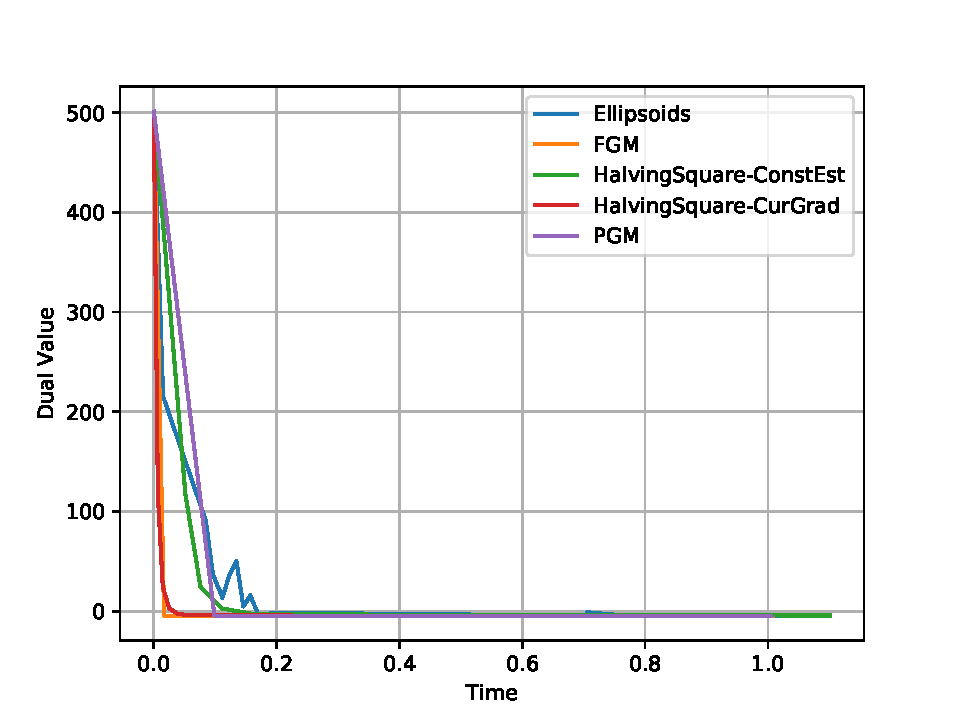
\includegraphics[width=0.7\linewidth]{Images/100_1e-03.pdf}} \\$n=100, \epsilon=1e-3$ \\
\end{minipage}
\hfill
\begin{minipage}[h]{0.47\linewidth}
\center{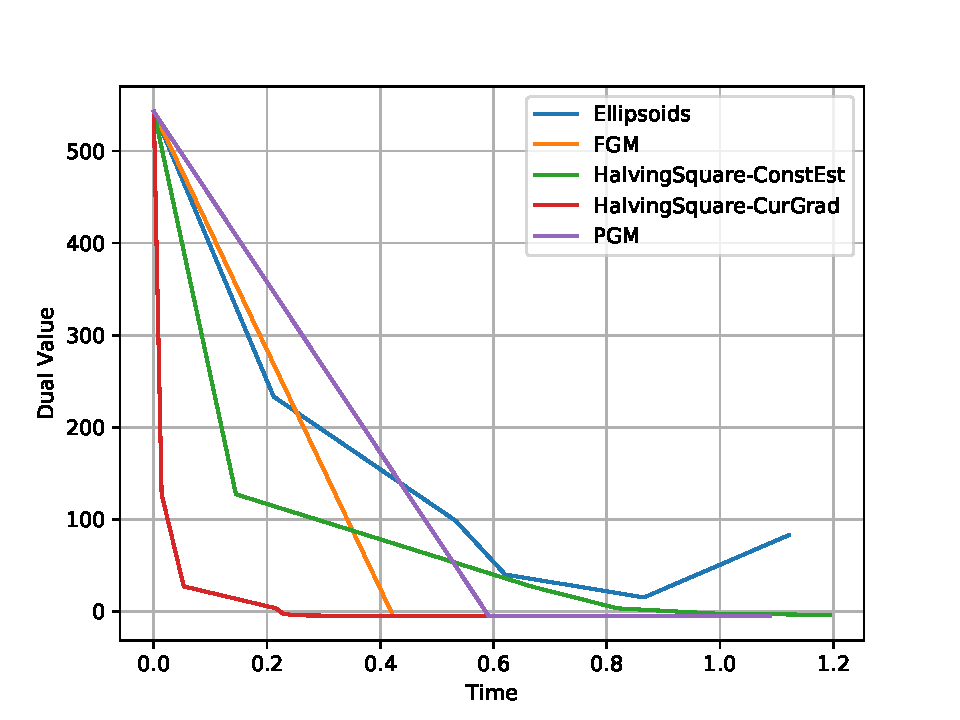
\includegraphics[width=0.7\linewidth]{Images/100_1e-10.pdf}} \\$n=100, \epsilon=1e-10$
\end{minipage}
\vfill
\begin{minipage}[h]{0.47\linewidth}
\center{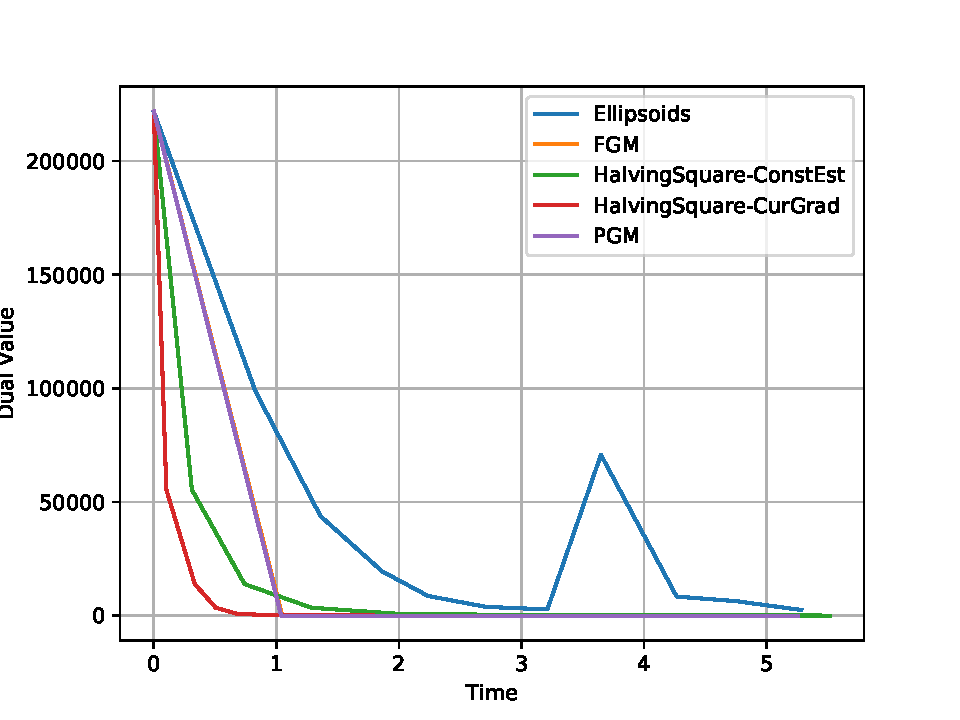
\includegraphics[width=0.7\linewidth]{Images/10000_1e-03.pdf}} \\$n=10000, \epsilon=1e-3$ \\
\end{minipage}
\hfill
\begin{minipage}[h]{0.47\linewidth}
\center{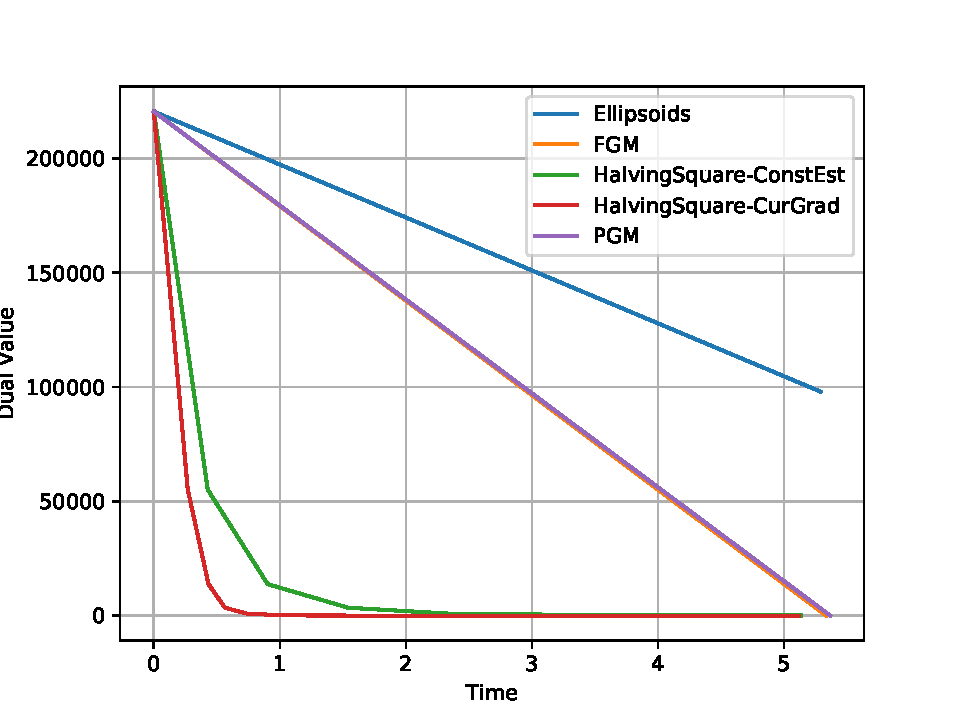
\includegraphics[width=0.7\linewidth]{Images/10000_1e-10.pdf}} \\$n=10000, \epsilon=1e-10$ \\
\end{minipage}
\end{figure}
\end{frame}

\section{Обобщение}

\begin{frame}{Обобщение}
Обобщение на случай размерности >2:
$$\text{Квадрат $\rightarrow$ $n$-мерный куб}$$
$$\text{Разделяющий отрезок $\rightarrow$ $n-1$-мерный гиперкуб}$$
\pause
Сходимость:
\begin{equation}N = \left\lceil\log_2\frac{La\sqrt{2n}}{\epsilon}\right\rceil.\end{equation}
\pause
Можно решать рекурсивно!
\end{frame}

\begin{frame}{Заключение}
\begin{itemize}
\item Метод двумерной оптимизации
\item Его приложение в решение двойственных задач
\item Превосходство стратегии CurGrad
\item Обобщение
\end{itemize}
\end{frame}


\begin{frame}
\center Спасибо за внимание!
\end{frame}

\end{document}


